\documentclass[../main.tex]{subfiles}

\begin{document}

%%%%%%%%%%%%%%%%%%%%%%%%%%%%%%%%%%%%%%%
%% Explain the block-matvec-product
%%%%%%%%%%%%%%%%%%%%%%%%%%%%%%%%%%%%%%%

\section{Handle memory issues with the interaction matrix}\label{sec:memory}

In the linear model with interactions, we need to build aforementioned
interactions.
We store them in the matrix $Z\in \bbR^{n\times q}$, with $q=\cO(p^2)$.
For large numbers of features $p$, it quickly becomes problematic to store
this data.
We thus consider a block approach that will only need to store a $n\times p$
matrix upmost at a time.
Indeed, we can decompose $Z$ into element-wise products with slices of $X$:
$Z=\begin{bmatrix}
		X \odot x_1 | X_{\llbracket 2,p \rrbracket} \odot x_2 |
		\cdots | X_{\llbracket p, p\rrbracket} \odot x_p
	\end{bmatrix}
	=\begin{bmatrix} Z_{\branch{q}{1}} |
		\cdots |Z_{\branch{q}{p}}
	\end{bmatrix}$.
So the product of $Z$ by a vector
$\Theta \in \bbR^{\nicefrac{p(p+1)}{2}}$ is:
 \[Z\Theta = \begin{bmatrix}
		Z_{\branch{q}{1}}\Theta_{\branch{q}{1}} +
		 \dots + Z_{\branch{q}{p}}\Theta_{\branch{q}{p}}\\
 \end{bmatrix} \enspace .\]

The first sum is a product with an $n\times p$ matrix,
the second sum is with a $n\times (p-1)$ matrix,
and so on until the last which is with a $n\times 1$ matrix.
Each block is computed efficiently using \texttt{CUDA} acceleration.

\medskip

For the product $Z^\top \xi$, $\xi\in\bbR^n$ (used in the gradient step),
we can also divide the blocks along the axis of size $q$.
Here, we sum over the axis of size $n$ which is quite large.
We can divide it to handle smaller reductions (see \Cref{fig:mat_trans}).
\begin{figure}[htbp]
	\centering
	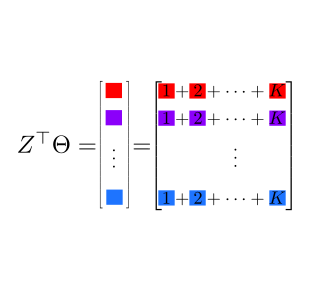
\includegraphics[scale=.35]{Ztranspose_matvec}
	\caption{Matrix-vector product for $Z^\top$ where $K$ should be big
	enough to avoid any error but
	also small enough to keep the power of a matrix product.}
	\label{fig:mat_trans}
\end{figure}

\noindent
And for each row, the $k^{th}$ sub-block, $1\leq k\leq K$ is computed as follows
(here for the first main row):
\begin{align*}
\displaystyle
\tikz[baseline]{
	\node[fill=red,anchor=base]{k};
	}
= \bigg[(Z_{\textcolor{red}{\branch{q}{1}}})^\top_{\llbracket n_k,n_{k+1}\rrbracket}
\xi_{\llbracket n_k,n_{k+1}\rrbracket}\bigg]
\enspace.
\end{align*}
For the $j^{th}$ main row, the first line uses the coefficients from $x_j\odot x_j$
but the last line always uses those from $x_j\odot x_p$.
Each sub-block $k$ is of size $n_k$ (for example the quotient of $n$ by $k$,
$\pm 1$ to reach $n$ at the end).

\paragraph*{Remark}
Having an efficient memory management is very important when working with GPUs.
There is very fewer available storage on a GPU than on a CPU.
Let us take as reference the NVIDIA GeForce RTX2080
(a standard graphical card that was used for the followings experiments).
The data can be stored in arrays (or tensor) of different types.
If stored with float-$32$, each element has a memory footprint of $4$ bytes.
In float-$64$, it is $8$ bytes.
The buffer memory of the GPU has $8GB$ available.
So for a float-$32$ tensor of size $n\times p$, we need
\[4np \leq 8\times 10^9 \Longrightarrow \sqrt{np} \leq 4.5\times 10^4\enspace.\]
And more generally considering the variance accross GPUs
(especially their date of release), we should have $\sqrt{np}\in [10000, 50000]$.
So the genomics data on which we will apply our methods (see \Cref{chap:genom})
generates a matrix $Z$ of size $20000\times 141246$ that does not fit.

\medskip

Recall that the algorithm we are trying to compete with
\citep{Bascou_Lebre_Salmon20} uses the \texttt{Numba} library to compile and
accelerate the code.
Now that we know how to make a matrix-vector product with the matrix $Z$, is
there a chance that, using GPU acceleration, we can perform operations faster
than \texttt{Numba}?
To see the time consumption of products of $Z$ with an array for different sizes,
we used the data from \Cref{chap:genom} with more than $19900$ samples and a large
number of features available.
We vary the number of features from $X$ and compute a product with the matrix $Z$
created on-the-fly.
We test it for \texttt{Numba} with a double loop (the way it is implemented in the
CD solver to update each coordinate).
We compare it with \texttt{PyTorch} using blocks (implemented for PGD/CBPG)
with and without \texttt{CUDA} to check that there is indeed an interest to
perform these operations with a GPU.
Also, because in the algorithms we use both products with $Z$ and $Z^\top$ and
the dimensions can be very different, we propose to monitor both.
Each operation has been repeated $20$ times.

\begin{figure}[ht]
	\begin{subfigure}{.45\textwidth}
		\centering
		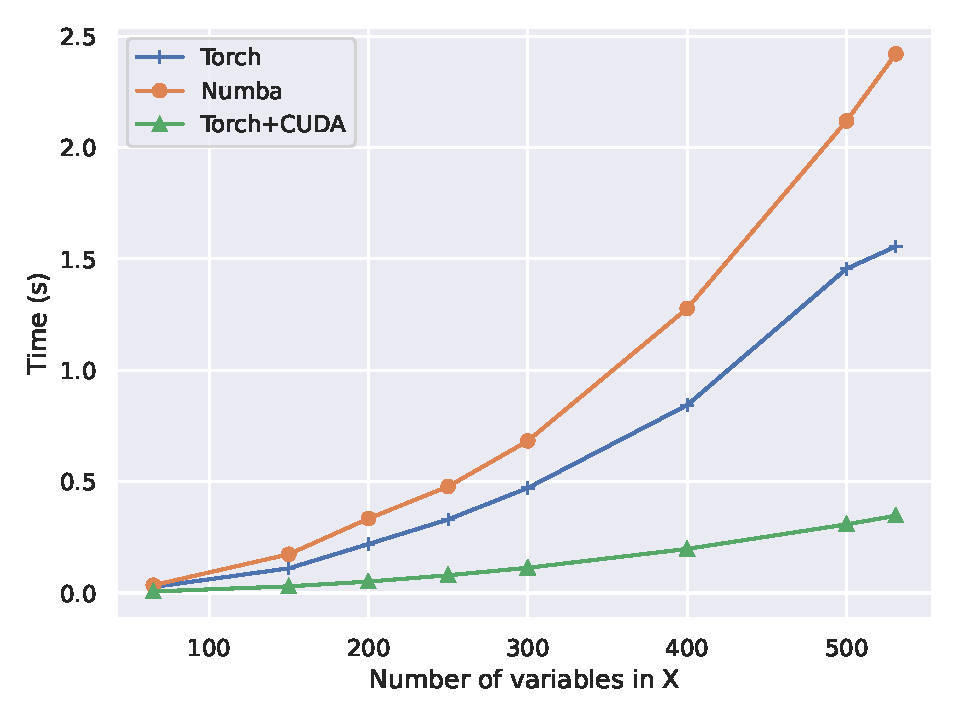
\includegraphics[width=\textwidth]{benchmark_prod_Zbeta}
		\subcaption{Product with the matrix $Z$.}
	\end{subfigure} \hfill
	\begin{subfigure}{.45\textwidth}
		\centering
		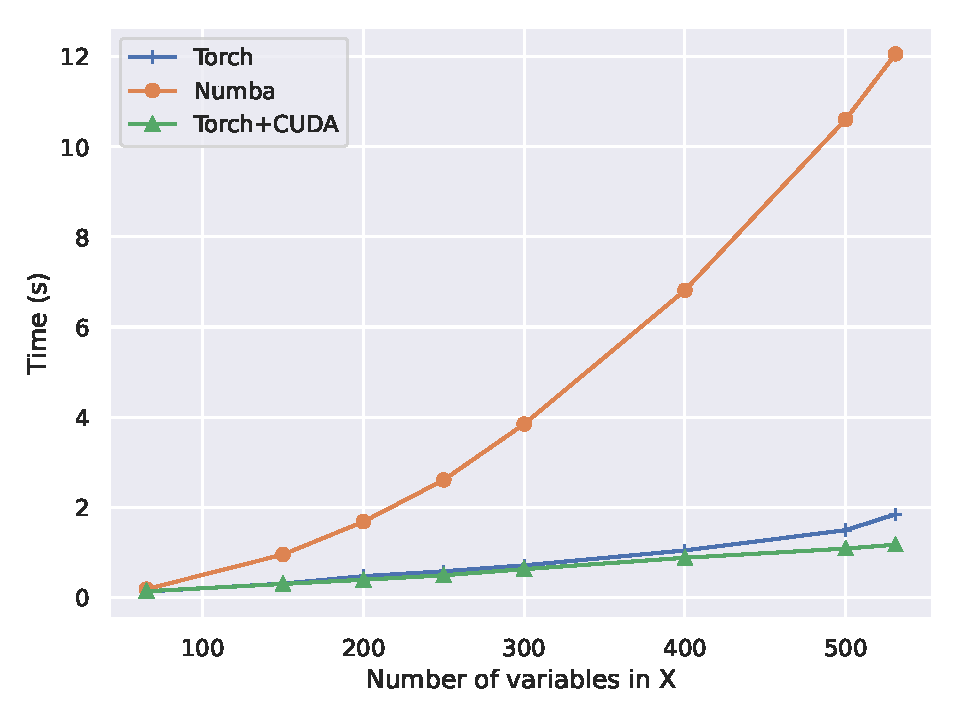
\includegraphics[width=\textwidth]{benchmark_prod_ZTtheta}
		\subcaption{Product with the matrix $Z^\top$.}
	\end{subfigure}
	\caption{
	Comparison on a genomics dataset of the median time to perform matrix
	vector products with the interaction matrix over $20$ repetitions.}
	\label{fig:matprod}
\end{figure}

\Cref{fig:matprod} shows us that indeed the time performance of matrix vector
products with \texttt{CUDA} as backend are performed way faster as the number
of features considered increases.
So can we actually increase the performance of Proximal Gradient type descent
algorithms this way? To answer this question, we still need some important
bricks to our foundations.
One of them being: at each step we want to move towards the solution:
but how do we choose the step size?

\section{Step-size for the interaction matrix}\label{sec:step_size}

One element needed for methods like PGD and CBPG is the computation of the step
size.
Essentially, we need to be able to compute or have a good upper bound for
$\norm{Z^\top Z}_2$ or for a fixed $i\leq p$,
$\bnorm{Z_{\branch{q}{i}}^\top Z}_2$.
To do so, several methods are available.
Below we present the one used.
We compare the upper bounds obtained with different methods.

\medskip

First in the PGD, for $\norm{Z^\top Z}_2$, we could simply use the power method
(Algorithm \ref{algo:pm}, \cite{golub2000eigenvalue}) to get the exact value.
This algorithm iterates through what is called the Krylov subspace of the
matrix $A$ and an associated vector $v_1$.
More formally, we denote the Krylov subspace of dimension $j\in\bbN^*$ $\cK_j(A, v_1)$
and define it as:
\begin{align*}
	\cK_j(A, v_1) = \span \left\{v_1, Av_1,\dots, A^{j-1}v_1\right\}
	\enspace.
\end{align*}

\begin{algorithm}[H]
	\label{algo:pm}
	\caption{Power method on a matrix $A$}
	\SetKwInOut{Input}{Input~}
	\SetKwInOut{Output}{Output~}
	\Input{$A\in \bbR^{n\times n}$, $m$ number of iterations}

	$v_1$ random unit vector

	\FOR{$j=1,\dots,m-1$}{
		$ v_{j+1} \longleftarrow Av_j$ \hspace{3cm}
		\textcolor{blue}{// visit a new direction} \\
		$ v_{j+1} \longleftarrow \frac{v_{j+1}}{\norm{v_{j+1}}}$ \hspace{2.5cm}
		\textcolor{blue}{// normalize the output}
	}

	\Output{$v_m$}
\end{algorithm}

However, using this method on CBPG with $p$ blocks becomes very costly
(especially considering that $Z_{\branch{q}{i}}^\top Z$ is not squared so we
have to apply the power method on $Z^\top Z_{\branch{q}{i}}Z_{\branch{q}{i}}^\top Z$).
An alternative is to consider not the exact value but an upper bound with
reasonable computation cost.
Such a bound could be computed from the consistency of the operator norm,
\ie $\bnorm{Z_{\branch{q}{i}}^\top Z}_2 \leq \bnorm{Z_{\branch{q}{i}}}_2 \bnorm{Z}_2$.

\begin{figure}[ht]
	\begin{subfigure}{.47\textwidth}
		\centering
		\includegraphics[width=\textwidth]{lipschitz_values_sklearndata}
		\subcaption{$p=150$ and $n=100$ on simulated dataset from the
		\texttt{make\_regression} function of \texttt{Scikit-learn}.}
	\end{subfigure} \hfill
	\begin{subfigure}{.47\textwidth}
		\centering
		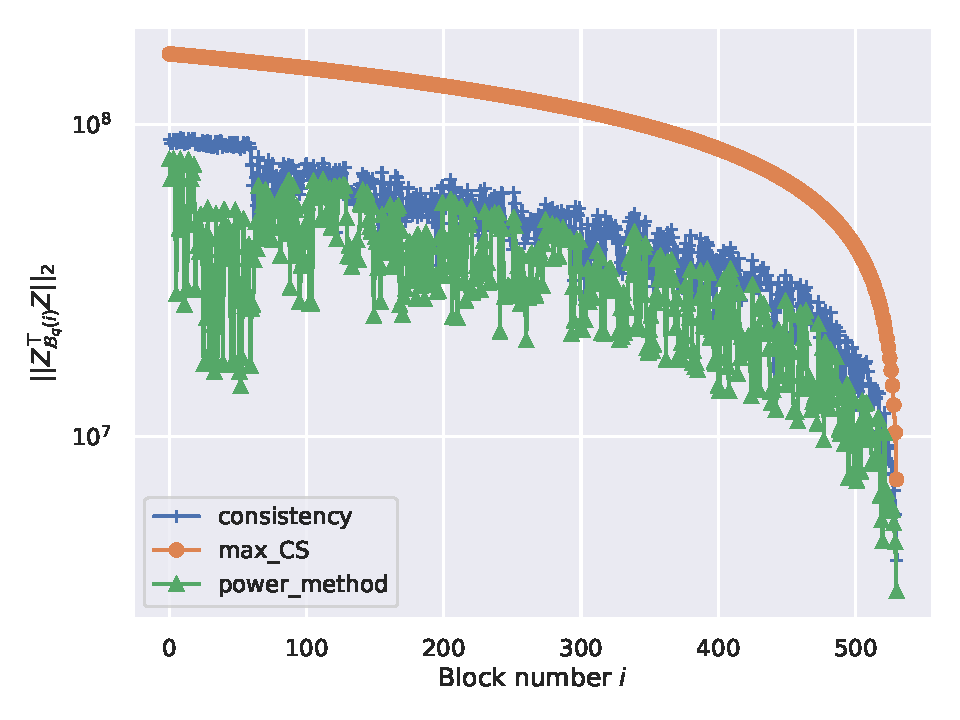
\includegraphics[width=\textwidth]{lipschitz_values_genomdata}
		\subcaption{$p=531$ and $n=19393$ on a genomics dataset
		(see \Cref{chap:genom})}
	\end{subfigure}
	\caption{Comparison of upper bounds on two datasets for
	$\norm{Z_{\branch{q}{i}}^\top Z}_2$.}
	\label{fig:lip_values}
\end{figure}

As we see in \Cref{fig:lip_values}, the upper bound produced can lead to quite
far results.
Those could imply very slow convergence (see \Cref{fig:importance_stepsize}).
Contrary to the power method, it is actually very fast to compute
an upper bound using the Cauchy-Schwarz inequality.
So it is reasonable for some situations to explain how to compute it.
\begin{figure}[h]
	\centering
	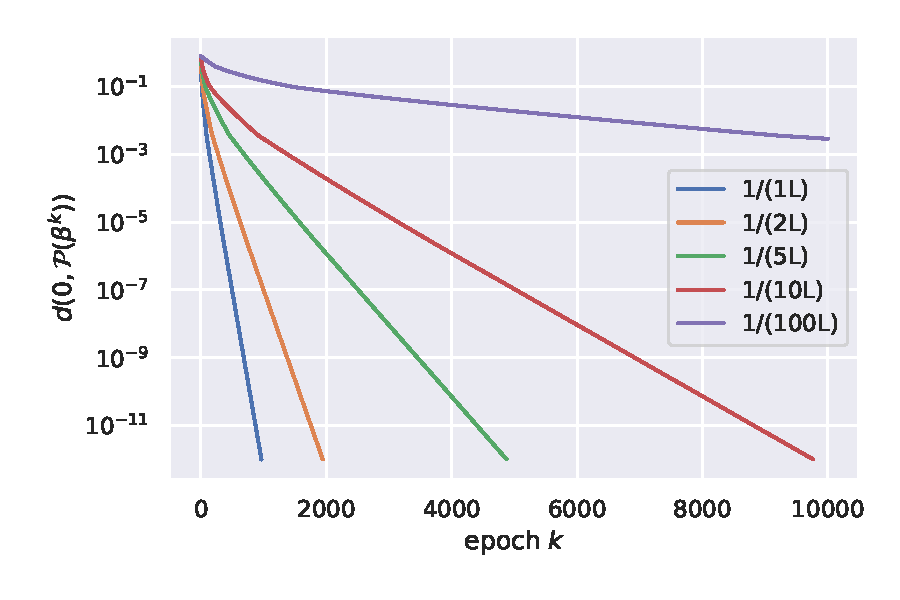
\includegraphics[scale=.55]{importance_step_size.pdf}
	\caption{
	Importance of the step size for ridge regularization (\texttt{Numpy}
	with \texttt{float}$64$ precision with $\lambda = 0.1$)
	on the Leukemia dataset ($n=72$, $p=7130$).
	$L$ is the Lipschitz constant $\nicefrac{\norm{X^\top X}_2}{n}$.
	The linear convergence rate (see \Cref{prop:ridge_kkt}) is obtained with steps
	near $L^{-1}$.
	Smaller steps lead to $\cO(\nicefrac{1}{k})$ convergence rates.
	}
	\label{fig:importance_stepsize}
\end{figure}

For the next part, recall that $Z\in\bbR^{n\times q}$ and
$Z_{\branch{q}{i}}\in\bbR^{n\times p_i}$.
For any matrix $K=(k_{ij})_{i,j}\in\bbR^{n_1\times n_2}$, we have
\citep[p.~27]{vandebril07}:
\begin{align}\label{eq:max_bound}
\norm{K}_2 \leq \sqrt{n_1n_2}\max_{i,j} |k_{ij}| \enspace.
\end{align}
Applying \eqref{eq:max_bound} to $K=Z_{\branch{q}{i}}^\top Z$, for each
$1\leq i\leq p$, we could compute $K$ by blocks and get the maximum component
each time.
But we can even go faster using Cauchy-Schwarz inequality.
Indeed, we want to perform our algorithms on the standardized matrix $Z$.
So for any $i$, $K$ is only a subset of the Gram matrix made from $Z$.
Thus for $l\in[p_i]$ and $m\in[q]$:
\begin{align*}
|k_{lm}| = \abs{
\left\langle Z_{\tau_q(i,l)}\, |\,  z_m\right\rangle
}
\leq \bnorm{Z_{\tau_q(i,l)}}_2 \bnorm{z_m}_2 \leq n
\enspace,
\end{align*}
because with a standardized matrix $Z$, $\norm{z_m}_2^2 = n \Var(z_m)=n$.
And this bound is reached when $\tau_q(i, l)=m$, so for each block
$Z_{\branch{q}{i}}$, we have:
\[\norm{Z_{\branch{q}{i}}^\top Z}_2 \leq n\sqrt{q p_i} \enspace.\]

The goal now is to improve the time consumption of the estimation of the largest
singular value without losing too much in precision.
We can indeed do better (see \Cref{fig:lanczos}) than the power method using the
L\'{a}nczos algorithm \Citep{lanczos1952solution} without diminishing the precision.
The core idea is quite simple. Where the power method iterates through the
Krylov space and only keeps the last iterate to generate a new direction,
L\'{a}nczos uses more deeply the Krylov space exploration made in all the past
iterations.
Note that this is not a method to directly compute the largest eigenvalue, but
more generally it is a way to approximate all of the extreme eigenvalues of a
(potentially very large) hermitian matrix by considering a smaller matrix $T$.
We have the relation \[T = V^* H V\enspace,\]
thus if $x$ is an eigenvector of a matrix $H$, then $Vx$ is an eigenvector of
$T$ for the same eigenvalue, where $V$ and $T$ are constructed by L\'{a}nczos
method.
\medskip

\begin{algorithm}[H]
	\label{algo:Lanczos}
	\caption{L\'{a}nczos algorithm on an hermitian matrix H}
	\SetKwInOut{Input}{Input~}
	\SetKwInOut{Output}{Output~}
	\Input{$H\in \bbR^{n\times n}$, $m$ dimension of the Krylov subspace visited}

	$v_1$ random unit vector

	\FOR{$j=1,\dots,m-1$}{
		$ w_{j+1} \longleftarrow Hv_j$ \hspace{3cm}
		\textcolor{blue}{// visit a new direction} \\
		$t_{k,j}  \longleftarrow \langle v_k, w_{j+1} \rangle,\ k=1,\dots, j$ \\
		$w_{j+1}  \longleftarrow w_{j+1} - \sum_{k=1}^j t_{k,j} v_k$
		\hspace{.8cm} \textcolor{blue}{// orthogonalization}\\
		$t_{j+1,j}\longleftarrow \|w_{j+1}\|_2$ \\
		$v_{j+1}  \longleftarrow \frac{w_{j+1}}{t_{j+1, j}}$
	}

	\Output{$T$}
\end{algorithm}

Algorithm \ref{algo:Lanczos} is quite general but shows that the basis fot this
method is indeed the power method, slightly modified.
In the case of $H$ hermitian, it is possible to show that $T$ is a tridiagonal
matrix.
Because it is an important result but not trivial just by looking at Algorithm
\ref{algo:Lanczos}, let us reprove it quickly by induction.
\begin{lemma}\label{lemma:lanczos}
The basis generated by the columns of $V$: $(v_1, \dots, v_m)_m$ is orthonormal.
\end{lemma}
\begin{proof}
The proof of this result can be written by induction.
Note that the fact that the columns of $V$ have unit norm is simply the last
line of the algorithm.
Let $v_1\in\bbR^n$ be a unit vector.
Then:
\begin{align*}
    \langle v_2, v_1 \rangle
    &= \left\langle \frac{w_2}{\norm{w_2}_2}, v_1\right\rangle \\
	&=\frac{1}{\norm{w_2}_2} \left\langle Hv_1 - \langle v_1, Hv_1\rangle
							  v_1, v_1\right\rangle\\
    &=\frac{1}{\norm{w_2}_2} \left\langle Hv_1, v_1\right\rangle -
	\frac{1}{\norm{w_2}_2}\left\langle v_1,Hv_1\right\rangle
	\underbrace{\norm{v_1}_2^2}_{=1} \\
    &= 0\enspace.
\end{align*}
If $(v_1,\dots, v_j)_{j\in\bbN^*}$ is an orthonormal basis,
then for $i\in[j]$,
\begin{align*}
    \langle v_{j+1}, v_i \rangle
    &=\frac{1}{\norm{w_{j+1}}_2}
		\left\langle Hv_j - \sum_{k=1}^j \langle v_k,
												 Hv_j\rangle
					 v_k, v_i\right\rangle \\
    &=\frac{1}{\norm{w_{j+1}}_2}
	\left[
		\left\langle Hv_j, v_i\right\rangle -
		\sum_{k=1}^j \langle v_k, Hv_j\rangle \left\langle v_k,
		 v_i\right\rangle
	\right]\enspace.
\end{align*}
Finally, we only need to notice that $\langle v_i, v_k\rangle = \norm{v_i}_2^2=1$
if $i=k$ and $0$ o.w. using to the induction hypothesis.
Thus $\norm{w_{j+1}}_2\langle v_{j+1}, v_i\rangle = \langle Hv_j,
 v_i\rangle - \langle v_i, Hv_j\rangle=0$.
So the columns of $V$ form an orthonormal basis of a subspace of the
Krylov subspace.
\end{proof}

To finalize, because we are in the Krylov subspace, the following relation is of
course verified:
\[\forall i < j-1,\exists \alpha_1, \dots, \alpha_k \in \bbR,\quad Hv_i =
\sum_{k=1}^{j-1} \alpha_k v_k\enspace. \]
Thus, using Lemma \ref{lemma:lanczos}
\begin{align*}
	t_{i, j} &= \langle v_i, w_{j+1}\rangle = 0,\ |i|<j-1,\\
	t_{j-1, j} &= \langle v_{j-1}, w_{j+1}\rangle = v_{j-1}^\top H v_{j}
	= v_{j}^\top H^\top v_{j-1} = \langle v_j, w_j\rangle = t_{j, j-1}
	\enspace.
\end{align*}
\begin{figure}[!h]
	\begin{subfigure}{.45\textwidth}
		\centering
		\includegraphics[width=\textwidth]{benchmark_powermethod_scipy}
		\caption{Time to produce the result (\texttt{PyTorch linalg} reference stops without
		possibility to stop)}
	\end{subfigure}\hfill
	\begin{subfigure}{.45\textwidth}
		\centering
		\includegraphics[width=\textwidth]{benchmark_powermethod_scipy_values}
		\caption{Difference with \texttt{linalg} reference value for our
		 iterative methods.}
	\end{subfigure}
	\caption{
	Comparison of the linalg module of \texttt{Pytorch}, the power
	method and L\'{a}nczos algorithms to get the largest singular value of an
	hermitian matrix with $n=20000$ and $500$ features.
	With same time performances L\'{a}nczos is much more precise faster.}
	\label{fig:lanczos}
\end{figure}
We simulate using standard gaussians $X \in \bbR^{n\times p}$ and
consider $H=X^\top X$.
We compare the time and precision for the power method, L\'{a}nczos algorithm
and \texttt{linalg} module of \texttt{PyTorch} to get $\|T\|_2$.
We consider several number of iterations for the power method,
and visit a subspace of same dimension with L\'{a}nczos method.
%
\section{Data types and GPU}
%
For our solvers, the CD method uses \texttt{Numba} with \texttt{Numpy}
as backend. Other solvers use \texttt{Pytorch} with \texttt{CUDA} enabled.
The steps are computed using the L\'{a}nczos method and after applying
$\texttt{linalg}$ function on the matrix $T$, with a subspace of dimension $20$.
\begin{figure}[!h]
	\centering
	\begin{subfigure}{.47\textwidth}
		\centering
		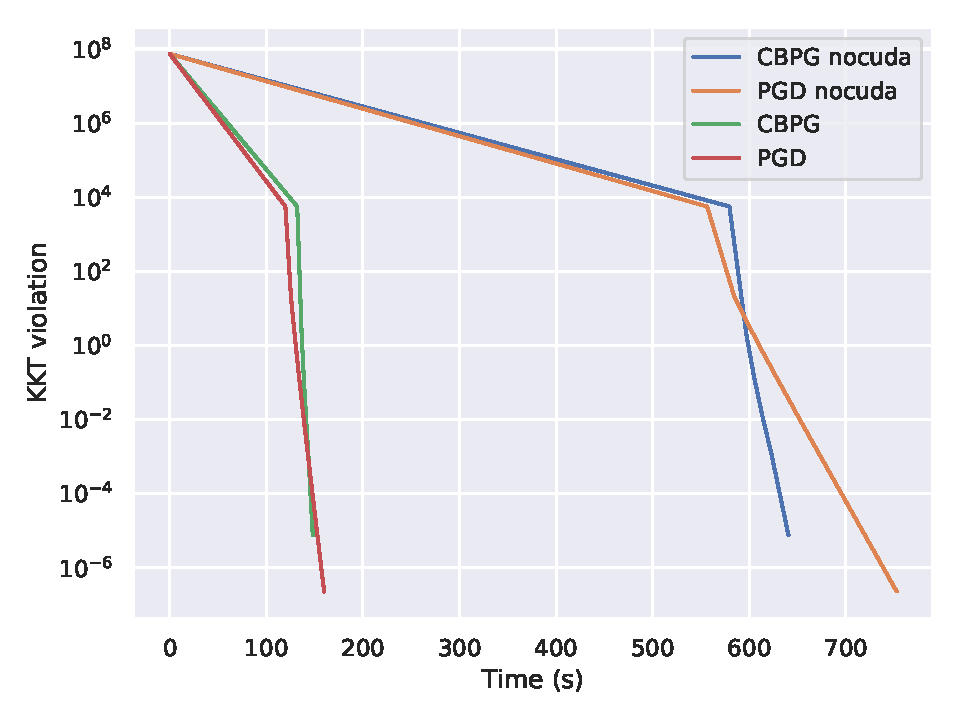
\includegraphics[width=\textwidth]{cuda_vs_nocuda_simulated_n20000p500}
		\subcaption{KKT violation criterion with CUDA vs no CUDA for PGD and
		CBPG with simulated data of $20000$ samples and $500$ features.}
		\label{fig:cuda_nocuda}
	\end{subfigure} \hfill
	\begin{subfigure}{.47\textwidth}
		\centering
		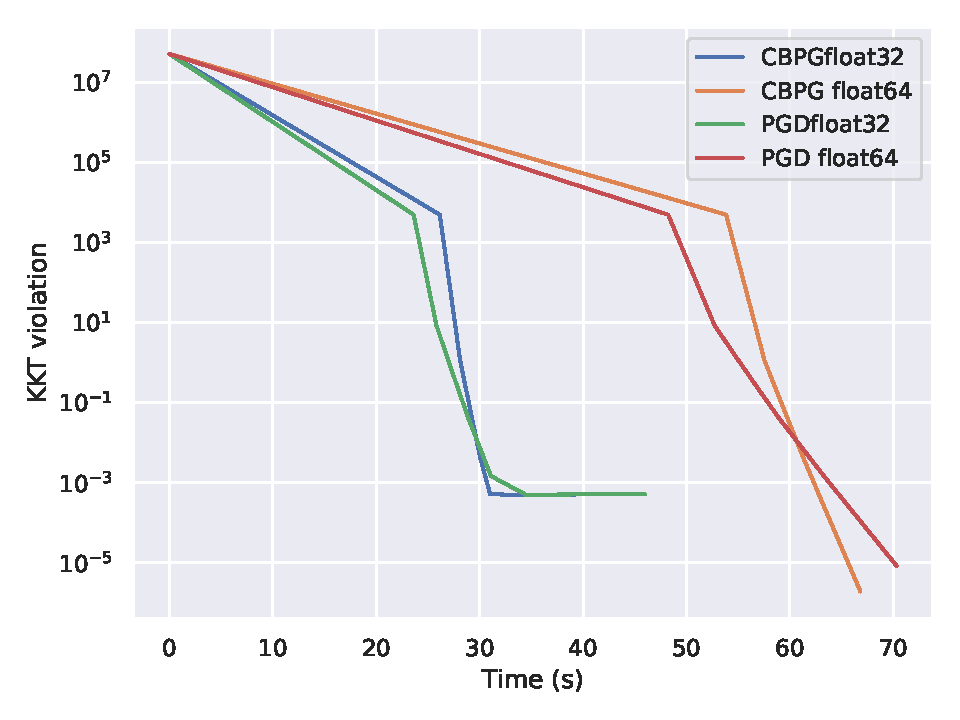
\includegraphics[width=\textwidth]{float_comparison_n25000p400}
		\subcaption{Effect of 32 or 64-bits precision on CBPG and PGD methods in
		a simulated dataset with $n=25000$ and $p=400$.}
		\label{fig:float}
	\end{subfigure}
	\caption{Comparison of data types and motivation to use
	\texttt{CUDA} acceleration.}
	\label{fig:floating_point}
\end{figure}

One can always wonder if there is an interest about using a more complex
architecture such as GPUs in this framework.
To test that, we simulated a dataset with $n=20000$, $p=500$.
We look at the difference between using \texttt{CUDA} or
stay purely on CPU for the PGD and CBPG methods.
It is clear from \Cref{fig:cuda_nocuda} that, when working with these solvers,
using GPU acceleration lead to results available in much fewer time.

\medskip

It is also well known and documented by libraries \citep{torch} that GPUs
should be used with \texttt{float32} precision for better performance.
However, our methods can accumulate some rounding errors that are amplified.
\Cref{fig:float} shows the time-precision trade-off we need to choose from in
our computation.
As a side-note, it should be noted that to this day in \texttt{Numba} when
accessing one coefficient from a \texttt{Numpy} array the type can be lost.
If the original array is in $32$-precision, the accessed values are casted
to $64$-precision internally because of \texttt{CPython}.

\section{Application to simulated dataset}

Simulated dataset entries are made from Gaussian variables. On KKT criterion
curves, if two consecutive values are close, then we stop the solver.
The signal to noise ratio is fixed.
For a random centered gaussian noise $\varepsilon$ of variance $\sigma^2$
and a target $y$, we use:
\[\mathrm{SNR} = \frac{\var(y)}{\sigma^2}\enspace.\]
We also need to choose the penalties. For that, let us first look at a upper
bound in our search.

\begin{definition}
	For the $\ell_1$ penalties, we denote $\lambda_{\max}>0$ the regularization
	such that
	\begin{align}
		\forall \lambda > \lambda_{\max},\  \beta=0_p \text{ and } \Theta=0_q
		\enspace.
	\end{align}
\end{definition}
%
It can be derived from the LASSO (see \Cref{sub:equivLasso} and
\citep{Fercoq_Gramfort_Salmon15}) that
\begin{align}
	\lambda_{\max} = \max\left(\frac{\norm{X^\top y}_\infty}{n},
							\frac{\norm{Z^\top y}_\infty}{n}\right)\enspace.
\end{align}
When a specific $\ell_1$ ratio is used (meaning the $\ell_1$ penalty is
$\alpha \ell_{1_\text{ratio}}$ and the $\ell_2$ penalty is
$\alpha(1-\ell_{1_\text{ratio}})$, $\alpha>0$), then
$\lambda_{\max}^{\text{ratio}}=\frac{\lambda_{\max}}{\alpha}$.

\medskip

\begin{figure}[!h]
	\centering
	\begin{subfigure}{.47\textwidth}
		\centering
		\includegraphics[width=\textwidth]{kkt_oban_simu_over10}
		\subcaption{$\ell_1$ regularizations are set to $\frac{\lambda_{\max}}{10}$
		and $\ell_2$ regularizations to $\frac{\lambda_{\ell_1}}{10}$.}
		\label{fig:simu_ccl}
	\end{subfigure} \hfill
	\begin{subfigure}{.47\textwidth}
		\centering
		\includegraphics[width=\textwidth]{kkt_simul_oban_over100}
		\subcaption{$\ell_1$ regularizations are set to $\frac{\lambda_{\max}}{100}$
		and $\ell_2$ regularizations to $\frac{\lambda_{\ell_1}}{10}$.}
		\label{fig:simu_ccl_over100}
	\end{subfigure}
	\caption{KKT criterion curves on the simulated regression dataset with
	$n=20000$ and $p=500$, $q=\nicefrac{p(p+1)}{2}$.
	Maximum number of epochs is set to $100$. Float types are $32$-bytes.
	}
\end{figure}

For now, we chose to use a simulated regression dataset with $p=500$ features
and $n=20000$. We also fixed the signal to noise ratio to $10$.
We denote the regularizations $\lambda_{\max}$ as the maximum between
$\lambda_{\Theta,\ell_1}$ and $\lambda_{\beta, \ell_1}$ ($\simeq 843.228$).

\medskip

As we see in \Cref{fig:simu_ccl}, Coordinate Descent is still faster for high
penalties. But decreasing the regularizations to $\nicefrac{\lambda_{\max}}{100}$
with the same signal to noise ratio leads to methods on GPU being equal or
faster than coordinate descent.
These simulations were made with a sparsity in $\beta$ and $\Theta$ of $25\%$
(meaning $25\%$ of the coefficients were active).
We wondered how sparser solutions could affect the solvers.

\begin{figure}[h]
	\centering
	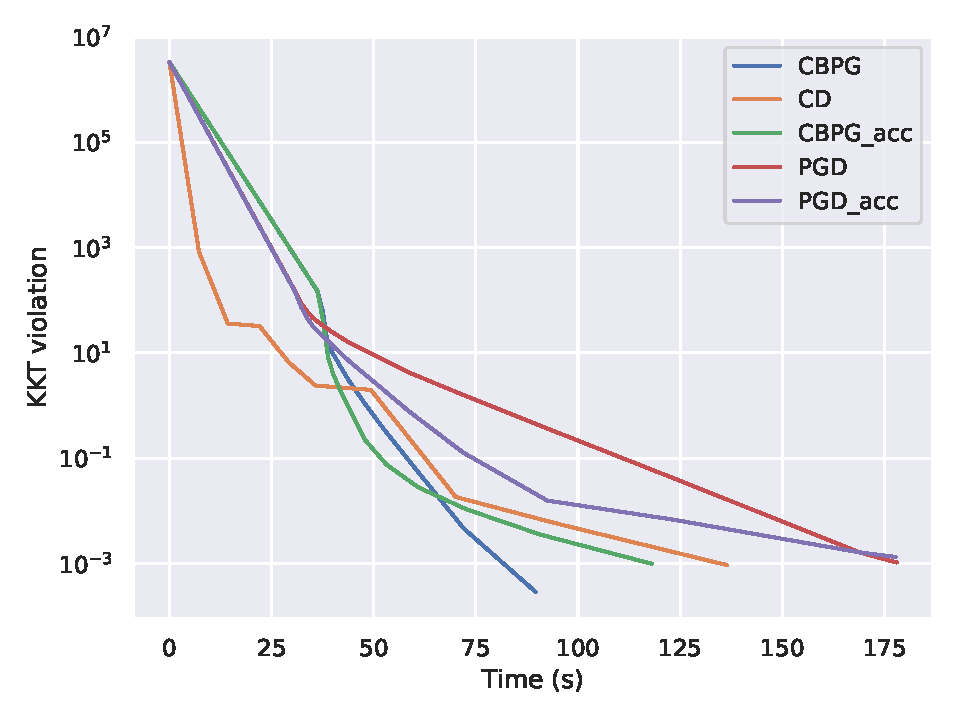
\includegraphics[scale=.5]{simulated_n20000p500_kkt_snr10_over100_sp}
	\caption{KKT criterion curves on the simulated regression dataset with
	$n=20000$, $p=500$
	Sparsity levels are set at $1\%$ in $\beta$ and $\Theta$.
	The $\mathrm{SNR}=10$, regularizations are set to $\frac{\lambda_{\max}}{100}$,
	Float-$32$ types are used and $100$ epochs are allowed.}
	\label{fig:sparsity_solvers}
\end{figure}

\medskip

With very sparse solutions, \Cref{fig:sparsity_solvers} shows that Coordinate
Descent methods have more advantages and lead over PGD. Here however CBPG
methods are still better.
We can wonder if dividing regularizations by such factors are realistic
(especially since we set the sparsity level to $1\%$ in our simulated dataset).
To investigate that we traced the surface plot
of the sparsity level obtained in the vector $\Theta$ (very large) against the
regularizations.
\Cref{fig:sp_surf} simply illustrates on an application how
important the choice of the LASSO penalty in the Elastic-Net is to get a good
sparsity level in the estimated coefficients.
We denote $\mathrm{nnz}(\Theta)=\# \{j\in[q]:\Theta_j\neq 0\}$.
%
\begin{figure}[!h]
	\centering
	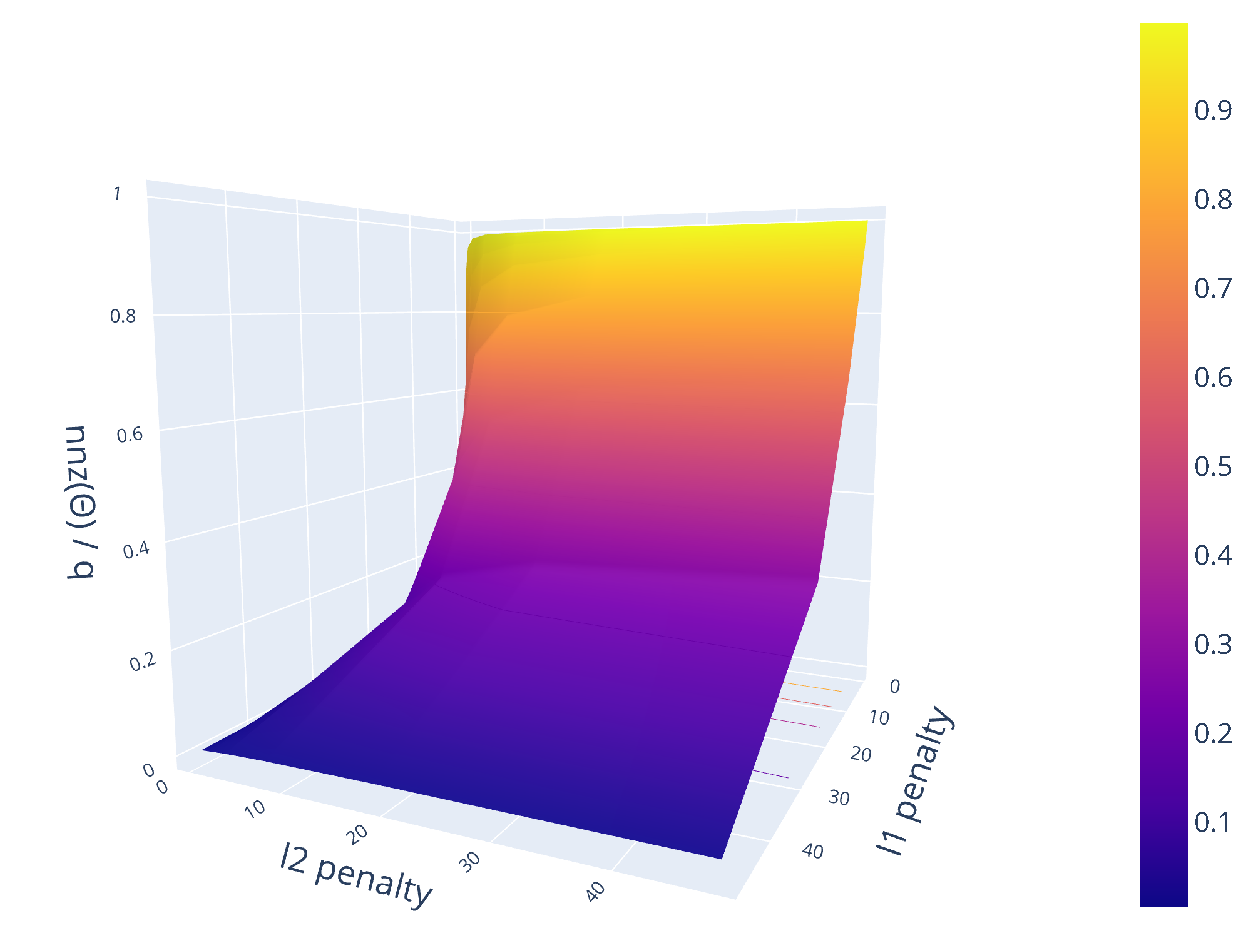
\includegraphics[scale=.4]{theta_surface_sparsity}
	\caption{Sparsity obtained in $\Theta$ with $n=20000$, $p=500$,
	$\mathrm{SNR}=10$, sparsity level simulated of $1\%$ in $\beta$ and
	$\Theta$, Float-$32$ types and $100$ epochs allowed.}
	\label{fig:sp_surf}
\end{figure}
%
The higher the $\ell_1$ penalty, the sparser the solution is and on datasets with
$p$ large, we want very sparse solutions.
For example, even having $1\%$ of non zero values for $p=500$ means around $1252$
active features in the interactions,
which in practice is still a lot and too difficult to interpret.

\medskip

We see that our GPU-accelerated methods are faster with smaller regularizations
and might seem not very useful, albeit it is not often that we know per advance
the right regularization to choose from.
In most cases, a set (or grid) of parameters is given to our method, we look at
the obtained Mean Squared Error (or any other criterion) and select the
regularization that lead to the best performance.
\begin{figure}[h!]
	\begin{subfigure}{.47\textwidth}
		\centering
		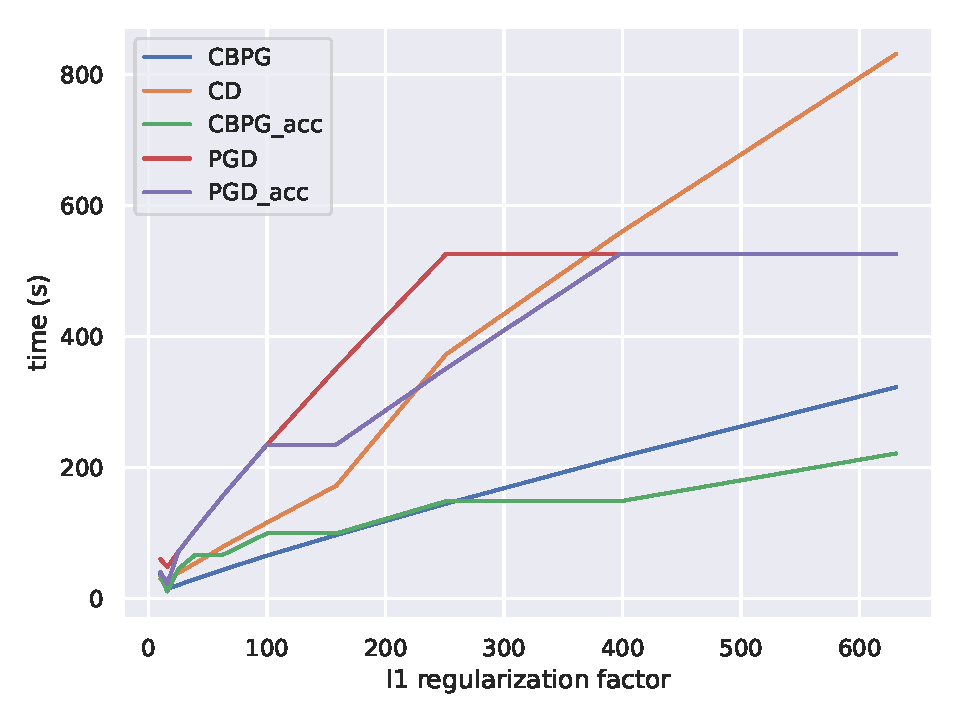
\includegraphics[width=\textwidth]{simulated_n20000p500_snr=10_TIME}
		\subcaption{Time consumption with varying $\ell_1$ penalty.}
		\label{fig:time_search}
	\end{subfigure} \hfill
	\begin{subfigure}{.47\textwidth}
		\centering
		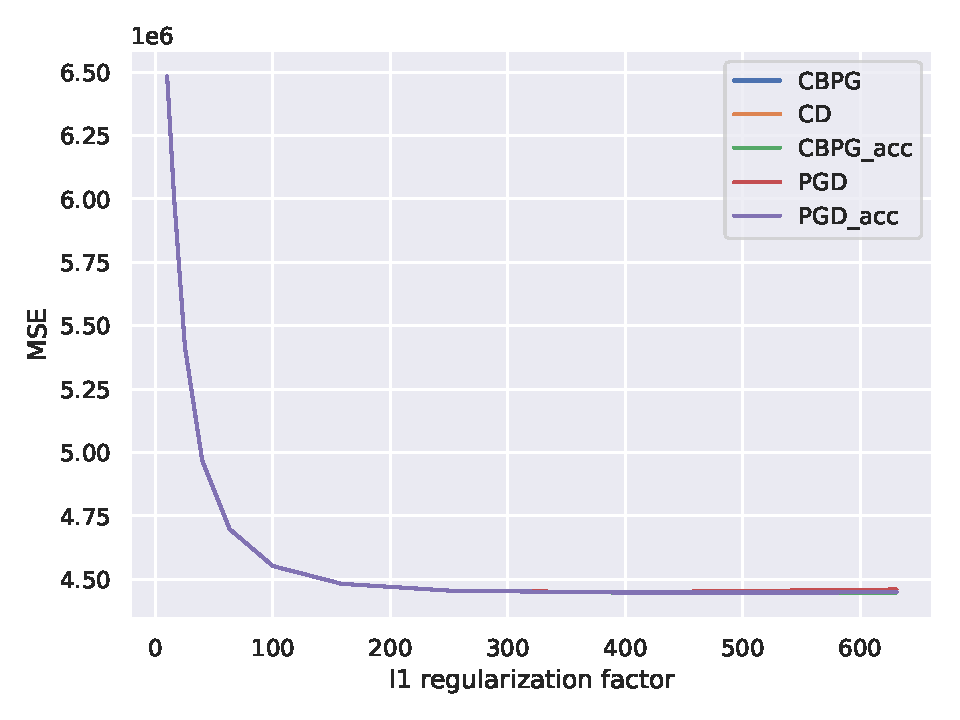
\includegraphics[width=\textwidth]{simulated_n20000p500_snr=10_MSE}
		\subcaption{MSE with varying $\ell_1$ penalty.}
		\label{fig:mse_search}
	\end{subfigure}
	\caption{On simulated regression dataset with $n=20000$ and $p=500$, $q=\frac{p(p+1)}{2}$.
	$\ell_1$ penalty is $\nicefrac{\lambda_{\max}}{\ell_1\text{factor}}$.
	Maximum number of epochs is set to $500$ but solvers stop if the criterion is achieved.
	Float types are $32$-bytes.
	KKT criterion is set to $10^{-3}$. SNR is set to $10$.
	Sparsity levels are at $1\%$.}
	\label{fig:path_simu}
\end{figure}
The key hypothesis is that we might not have any prior idea about the location
of the best parameters. In this situation, one can choose a grid search of
$\nicefrac{\lambda_{\max}}{\ell_1\ \text{factor}}$ for the $\ell_1$ regularization.
Let us use $\lambda_{\ell_2}=\frac{\lambda_{\max}}{10}$ and see for varying
$\ell_1$ regularizations the time spent and the MSE obtained.
Also, doing so we don't need to compute each time the Lipschitz constants of
all the blocks in the Cyclic Block method, they are computed for one run and
the next ones can reuse them.

\medskip

As we see in \Cref{fig:mse_search} all our errors are close.
And with \Cref{fig:time_search} we see the three situations we encountered before.
Around a division of $\lambda_{\max}$ by $10$ and before, CD is faster.
After that CD is better than PGD-type methods but not CBPGs.
And then it needs to search even longer.
Note that in this experiment, only PGD methods did not reach the $\epsilon=10^{-3}$
precision in the $500$ epochs allowed for the last regularizations.
Hence the flattening curve meaning we only see the time it takes to make the
maximum number of epochs.
And although it appears the MSE curve is strictly decreasing,
in fact the MSE for the last regularization is higher than the one for
the penultimate's.

\paragraph*{With warmstart and residuals recomputation}
We describe in \Cref{sec:solv_genom} ways to reach lower precision.
The warmstart uses solutions from one penalty to be injected as first guess
for the next penalty.
Using a $\ell_1$ ratio of $0.9$ we can, on simulated data,
compute a path and compare times to reach a precision of $10^{-4}$
(see \Cref{fig:path_genom}).

\begin{table}[ht]
    \caption{Non zero values in $\beta$ and $\Theta$ from the simulate experiment
	of \Cref{fig:path_genom}. Both methods lead to the same results.
	The $\ell_1$ ratio is set to $0.9$. Higher values of $\alpha$ lead to
	$\lambda_{\beta, \ell_1}$ and $\lambda_{\Theta,\ell_1}$ larger and result
	to fewer features selected.}
	 \label{tab:nnz}
    \centering
    \begin{tabular}{lcccccccccc}
        \hline
        $\alpha$& 851.7 & 516.1 & 312.6 & 189.4 &
        114.8 & 69.5 & 42.1 & 25.5 &  15.5 & 9.4 \\\hline
        $nnz(\beta)$  & 1 & 4 & 5 & 5 & 5 & 5 & 22 & 53 & 93 & 124 \\
        $nnz(\Theta)$ & 0 & 0 & 0 & 0 & 89 & 706 & 5068 & 13899 & 22844 & 29767
		 \\\hline
    \end{tabular}
\end{table}
Both solvers keep the same number of non zeros coefficients (see \Cref{tab:nnz})
and result to the same MSE.
We could also consider different values for the $\ell_1$ ratio and more values
of $\alpha$ in the grid to select the penalties resulting with the least MSE
on the test set.
\begin{figure}[!h]
    \centering
    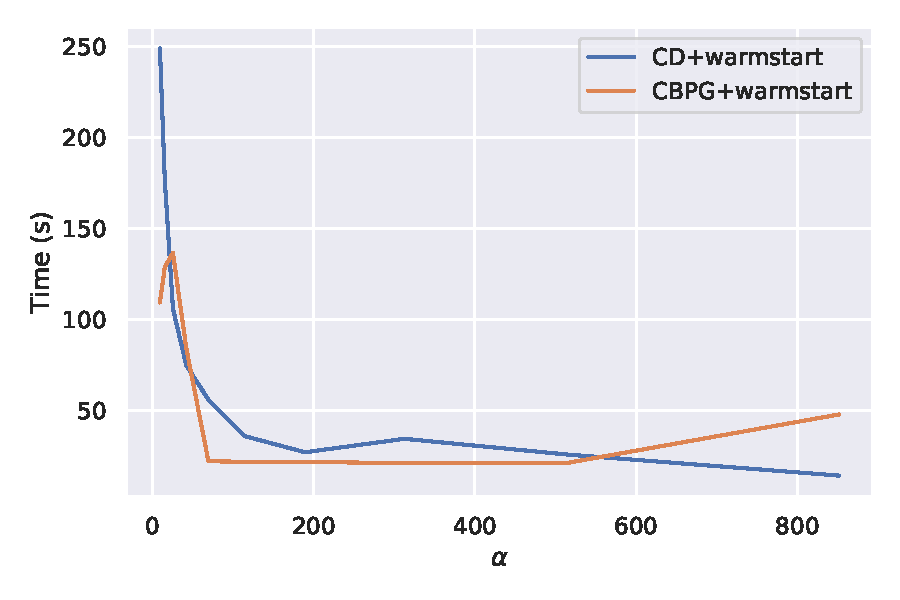
\includegraphics[scale=.6, clip, trim={0cm 0cm 15cm .5cm}]{simu_ratio09}
    \caption{Use of the recomputation of the residuals on simulated dataset
	with a $\ell_1$ ratio of $0.9$, $n=20000$, $p=500$ ($15000$ samples for the
	train phase and the rest for the test), $1\%$ of non zero values in the
	coefficients vectors and solvers are stopped when the KKT criterion reaches
	$10^{-4}$. The $\ell_1$ penalty is $\alpha\ell_1{_{\text{ratio}}}$ with
	$10$ values of $\alpha\in[\lambda_{\max}/100, \lambda_{\max}/1.1]$
	$\log$-spaced (consider $\lambda_{\max}$ as upper bound would lead to
	zero-filled vectors which is not interesting).}
    \label{fig:path_genom}
\end{figure}

\medskip

Note that in this situation, for the last penalty
($\alpha = 10^{-2}\lambda_{\max}$) which is
the hardest to compute, both solvers converged.
Coordinate Descent reached $10^{-4}$ precision in $21$ epochs,
 and Coordinate Block Gradient Descent in $57$ epochs.
So more than twice the number of epochs, only each one is done
faster thanks to the GPU so \emph{in fine} and counterintuitively, the method
doing more epochs is faster.

\end{document}
